\documentclass{parcfd2015}

\usepackage{graphicx}
\usepackage{amsmath}
\usepackage{amsfonts}
\usepackage{amssymb}

\title{PetIBM - A PETSc-based Immersed Boundary Method code}

\author{OLIVIER P. MESNARD$^{*}$, ANUSH KRISHNAN$^{*}$ \\ AND LORENA A. BARBA$^{*}$}

\heading{Olivier P. Mesnard, Anush Krishnan and Lorena A. Barba}

\address{$^{*}$ Mechanical and Aerospace Engineering, The George Washington University\\
Washington, DC, 20052, United-States\\
e-mail: mesnardo@gwu.edu, web page: lorenabarba.com}

\keywords{Immersed Boundary Method, PETSc, flying snake}

\abstract{A new, open-source \texttt{PETSc}-based immersed boundary method code is under development that uses a fully discrete projection formulation. Its initial purpose is to study the three-dimensional flow around an accurate cross-sectional shape of the flying snake species \textit{Chrysopelea paradisi}. We analyze vorticity structures in the wake and explain the enhanced lift generation of the snake at a particular angle of attack.}

\begin{document}
\maketitle

\section{IMMERSED BOUNDARY METHOD}

Immersed boundary methods (IBM) form a class of techniques in computational fluid dynamics where an immersed boundary is represented by a collection of Lagrangian points that do not coincide with the Eulerian grid nodes. They are particularly useful to simulate flows over complex and moving geometries. Simple, structured Cartesian meshes covering the entire physical domain (including the solid region) can be used, requiring low memory storage. The governing equations are solved over the whole domain and the key is finding a way to incorporate the boundary conditions on the immersed surface.

We use the method proposed by Taira and Colonius \cite{Taira_Colonius_2007} in which the momentum equations are augmented by a forcing term that acts as a Lagrange multiplier to bring the fluid to rest in the vicinity of the body surface. The fully-discrete modified Navier-Stokes equations produce an algebraic system that is solved via a projection method by performing a block LU decomposition \cite{Perot_1993}.

\section{PETIBM}

We use the open-source library \texttt{PETSc} \cite{PETSc_webpage_2014} to build the IBM code, taking advantage of its efficient data structures and routines to solve partial differential equations on multi-CPUs. The \texttt{PETSc} data structure \textit{distributed array} allows us to perform a logically Cartesian decomposition, such that nodal values spatially close in the physical domain are stored on the same process, thus, minimizing communications when using finite-difference stencils. Explicit terms of the Navier-Stokes system are stored using \textit{local vectors} that include ghost-cell values while \textit{global vectors} are used in sparse linear algebra routines.

The full code, named \texttt{PetIBM}, is open-source, released under an MIT License and hosted on the version-controlled platform GitHub \cite{PetIBM}.

\section{APPLICATION TO FLYING SNAKES}

We study the aerodynamics of the \textit{Chrysopelea paradisi}, a species of flying snake. Previous experimental work \cite{Holden_et_al_2014} reported enhanced lift force on a snake gliding at angle of attack of $35^o$ for flows with Reynolds number beyond $9000$. Two-dimensional numerical investigations confirmed a spike in the lift curve at this particular angle of attack ($Re=2000$) \cite{Krishnan_et_al_2014}. Using \texttt{PetIBM}, we aim to understand the three-dimensional wake structures responsible for high gliding performances of the paradise tree snake.

\begin{figure}[h!]
\centering
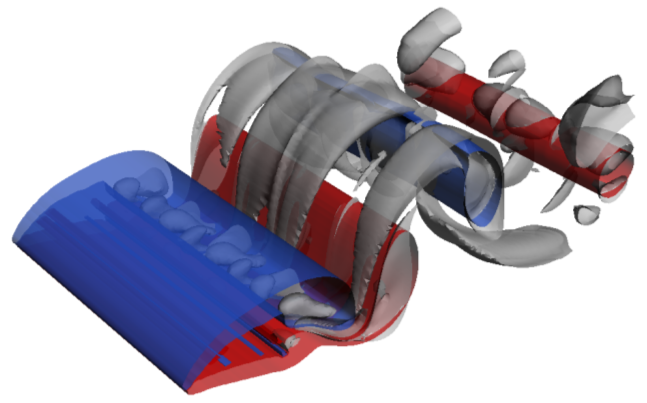
\includegraphics[width=8cm]{images/flying_snake_petibm.png}
\caption{Contours of the spanwise (red and blue) and streamwise (grey) components of the vorticity shed in the wake of an infinitely long cylinder with cross-section of the \textit{Chrysopelea paradisi}.}
\label{flying_snake_petibm}
\end{figure}

\begin{thebibliography}{99}
\bibitem{PETSc_webpage_2014} Balay S., Abhyankar S., Adams M.F., Brown J., Brune P., Buschelman K., Eijkhout V., Gropp W.D., Kaushik D., Knepley M.G., Curfman McInnes L., Rupp K., Smith B.F. and Zhang H. PETSc Web page. \texttt{http://www.mcs.anl.gov/petsc} (2014).
\bibitem{Holden_et_al_2014} Holden D., Socha J.J., Cardwell N.D. and Vlachos P.P. Aerodynamics of the flying snake Chrysopelea paradisi: how a bluff body cross-sectional shape contributes to gliding performance. \textit{J. Exp. Biol.} (2014) \textbf{217}:382--394.
\bibitem{PetIBM} Krishnan A. and Barba L.A. PetIBM - A 3D and parallel PETSc-based immersed boundary method code. \texttt{https://www.github.com/barbagroup/PetIBM}.
\bibitem{Krishnan_et_al_2014} Krishnan A., Socha J.J., Vlachos P.P. and Barba L.A. Lift and wakes of flying snakes. \textit{Phys. Fluids} (2014) \textbf{26(3)}:031901.
\bibitem{Perot_1993} Perot J.B. An analysis of the fractional step method. \textit{J. Comp. Phys.} (1993) \textbf{108(1)}:51--58.
\bibitem{Taira_Colonius_2007} Taira K. and Colonius T. The immersed boundary method: A projection approach. \textit{J. Comp. Phys.} (2007) \textbf{225(2)}:2118--2137.
\end{thebibliography}

\end{document}


